%==============================================================================
\chapter{Randbedingungen}
\label{chap:param}
%==============================================================================

In diesem Kapitel werden die Randbedingungen der in Kapitel \ref{chap:methodik} definierten physikalischen Modelle der Kraftstoffsysteme festgelegt. Ziel ist es, das Verhalten der Kraftstoffsystemen im Reiseflug möglichst realitätsnah abzubilden. Anhand der Parameter werden die Kraftstoffsysteme für die Triebwerke eines Schmalrumpfflugzeugs dimensioniert. Zunächst werden die relevanten Betriebspunkte der verwendeten Triebwerkszyklen beschrieben. Hierauf werden die relevanten Parameter bestimmt und deren Herkunft erläutert. Abschließend werden die unabhängigen Variablen der Kraftstoffsysteme parametriert und für die Wasserstoff-Kraftstoffsysteme Wertebereiche für die Parameterstudie festgelegt.

\section{Triebwerkszyklus}

Die Dimensionierung der Komponenten und die Bestimmung der Randbedingungen der Kraftstoffsysteme erfolgt auf Grundlage von Triebwerkszyklen für moderne wasserstoff-/kerosinbetriebene Getriebefantriebwerke (engl.: Geared Turbo Fan, GTF) für Schmalrumpfflugzeuge, in Anlehnung an das Pratt \& Whitney PW1133G Triebwerk. Die Betriebspunkte der Triebwerkszyklen wurden am IST mit GasTurb \cite{GasTurbGmbH.2021}, einer Software für die Gasturbinen-Leistungsrechnung, berechnet. Der Betriebspunkt für den Reiseflug wurde für die beiden Zyklen bei einer Flughöhe von \SI{10700}{\m}, einer Machzahl von 0,78, unter Annahme der Internationalen Standardatmosphäre (ISA) und einem Schub von \SI{22}{\kilo\N} gerechnet. Die für den Reiseflug berechneten Werte sind in Tabelle \ref{Tab:cruise} zusammengefasst.

\begin{table}[ht]
    \centering
	\caption{Betriebspunkt Reiseflug}
	\begin{tabular} {|l|c|c|c|c|} \hline%
    \multicolumn{2}{|c|}{Parameter} & Einheit & H\textsubscript{2} & Kerosin \\ \hline\hline%
    Schub & $F$ & kN & \multicolumn{2}{c|}{22} \\ \hline
    Flughöhe & $H$ & m & \multicolumn{2}{c|}{10.700} \\ \hline
    Machzahl & $M$ & - & \multicolumn{2}{c|}{0,78} \\ \hline
    Umgebungstemperatur & $\Delta T_{\mathrm{ISA}}$ & K & \multicolumn{2}{c|}{0} \\ \hline\hline
    Kraftstoffmassenstrom & $\dot{m}_\mathrm{BK}$& kg/s & 0,110 & 0,313 \\ \hline
    Hochdruckwellendrehzahl & $N_2$ & 1/min & \multicolumn{2}{c|}{19.000} \\ \hline
    Niederdruckwellendrehzahl & $N_1$ & 1/min & \multicolumn{2}{c|}{9000} \\ \hline
    Fan-Drehzahl & $N_\mathrm{F}$ & 1/min & \multicolumn{2}{c|}{3000} \\ \hline
    Brennkammerdruck & $p_3$ & kPa & \multicolumn{2}{c|}{1330} \\ \hline
    Fan-Zapflufttemperatur & $T_{13}$ & K & \multicolumn{2}{c|}{273} \\ \hline
    %Umgebungstemperatur & $T_\mathrm{U}$ & K & 219 & - \\ \hline
    Fan-Leistung & $P_\mathrm{F}$ & kW & \multicolumn{2}{c|}{6400} \\ \hline
    \end{tabular}	
    \label{Tab:cruise}%
\end{table}
\FloatBarrier 

Für die Dimensionierung der Hochdruckpumpe des Kerosin-Kraftstoffsystems ist neben dem Reiseflug auch der Betriebspunkt mit maximalem Startschub (engl.: Maximum Takeoff, MTO) von Interesse. Der Betriebspunkt für den Startfall wurde für den Kerosin-Triebwerkszyklus bei einer Flughöhe von $0$ m, einer Machzahl von $0$, unter Annahme von ISA-Bedingungen und mit dem MTO-Schub von $147$ kN gerechnet. Die für die Arbeit relevanten berechneten Werte sind in Tabelle \ref{Tab:mto} gelistet.

\begin{table}[ht]
    \centering
	\caption{Betriebspunkt MTO-Schub}
	\begin{tabular} {|l|c|c|c|} \hline%
    \multicolumn{2}{|c|}{Parameter} & Einheit & Kerosin \\ \hline\hline%
    Schub & $F$ & kN & 147 \\ \hline
    Flughöhe & $H$ & m & 0 \\ \hline
    Machzahl & $M$ & - & 0 \\ \hline
    Umgebungstemperatur & $\Delta T_\mathrm{ISA}$ & K & 0 \\ \hline\hline
    Kraftstoffmassenstrom & $\dot{m}_\mathrm{BK}$& kg/s & 1,05  \\ \hline
    Hochdruckwellendrehzahl & $N_2$ & U/min & 21.000 \\ \hline
    \end{tabular}	
    \label{Tab:mto}%
\end{table}
\FloatBarrier 

\section{Eintrittsbedingungen}

Die Kraftstoff-Eintrittstemperatur in Kerosin-Kraftstoffsystemen wird maßgeblich von der Umgebungstemperatur, der verbleibenden Kraftstoffmenge, der Flugdauer sowie der durch Rezirkulation in die Kraftstofftanks rückgeführten Wärme beeinflusst \cite{German.2012}. In dieser Arbeit wird für das Kerosin-Kraftstoffsystem eine Kraftstoff-Eintrittstemperatur von $T_\mathrm{e}=$ \SI{270}{\K} angenommen, was in einer Flughöhe von $H= $ \SI{10700}{\m} einer um \SI{51.3}{\K} höheren Temperatur im Vergleich zur Umgebungstemperatur entspricht. 

Gemäß der Musterzulassung des Pratt \& Whitney PW1133G Triebwerks darf der Eintrittsdruck $p_\mathrm{e}$ einen Überdruck von \SI{689}{\kilo\Pa} relativ zur Umgebung nicht überschreiten und einen Überdruck von \SI{34.5}{\kilo\Pa} zum Dampfdruck des Kraftstoffs nicht unterschreiten \cite{EASA.2018}. Bei einer Kraftstoffeintrittstemperatur von $T_\mathrm{e}=$ \SI{270}{\K} und einer Flughöhe von \SI{10700}{\m} entspricht dies einem Druckbereich von \SI{35.0}{\kilo\Pa} bis \SI{713}{\kilo\Pa}. Durch den Förderdruck der verwendeten Boosterpumpe von ca. \SI{250}{\kilo\Pa} \cite{EatonFuelSystemsDivision.2013} ist dem Kraftstoffeintrittsdruck eine engere Obergrenze gesetzt. Abzüglich Rohrreibungsverlusten in den Kraftstoffleitungen zwischen Kraftstofftank und Triebwerk wird ein Eintrittsdruck von $p_\mathrm{e}=$ \SI{180}{\kilo\Pa} angenommen.

Das von Brewer \cite{Brewer.1991} vorgeschlagene Kraftstoffsystem, an dem sich die Wasserstoff-Kraftstoffsysteme dieser Arbeit orientieren, verwendet einen Flüssigwasserstofftank mit einem absoluten Druck von \SI{152}{\kilo\Pa} sowie eine im Tank integrierte Niederdruckpumpe, die den flüssigen Wasserstoff auf \SI{462}{\kilo\Pa} fördert. Die Autoren des CRYOPLANE-Berichts \cite{Scholz.2003} treffen ähnliche Annahmen. Unter Berücksichtigung von Druckverlusten erreicht der Wasserstoff das Triebwerk mit einem Eintrittsdruck von $p_\mathrm{e}=$ \SI{345}{\kilo\Pa} \cite{Brewer.1991}. Die von Brewer ermittelte Wasserstoff-Eintrittstemperatur $T_\mathrm{e}=$ \SI{25.2}{\K} entspricht dem Siedepunkt von Parawasserstoff. In dieser Arbeit wird für den Eintritt eine rein flüssige Wasserstoffphase angenommen.

\section{Abwärmequellen}

Zur Berechnung der in den Wärmeübertragern der Kraftstoffsysteme übertragenen Wärmeströme werden die in den Triebwerken entstehenden Abwärmeströme aufsummiert. Zu den Abwärmequellen moderner Gasturbinentriebwerke zählen neben den Komponenten des Hilfsgeräteträgers insbesondere die Wellenlager sowie, falls vorhanden, das Fan-Getriebe (engl.: Fan Drive Gear System, FDGS). Dem Wasserstoff-Kraftstoffsystem steht in Form eines Wärmeübertragers mit dem Kabinen-Klimasystem (ECS) eine zusätzliche Abwärmequelle zur Verfügung. 

\subsection{Wellenlager}

Die Wellenlager sind eine Quelle mechanischer Verluste und übertragen die verlorene Leistung nahezu vollständig an das Ölsystem \cite{Gloeckner.2017}. Das PW1133G Triebwerk ist mit sieben Wellenlagern ausgestattet: Die Hochdruckwelle wird durch ein Fest- und ein Loslager gelagert, die Niederdruckwelle durch ein Fest- und zwei Loslager, und die Fan-Welle wird durch eine angestellte Lagerung gestützt \cite{AviationKnowledge.2022}. 

Die Lagerverluste hängen in erster Linie von der Wellendrehzahl ab, wobei bei Festlagern auch die axiale Belastung der Welle einen Einfluss hat \cite{Zhao.2023}, die in dieser Betrachtung jedoch vernachlässigt wird. Gloeckner et al. \cite{Gloeckner.2017} haben für ein Hochdruckwellenlager bei einer Drehzahl von $19.000$ 1/min einen Leistungsverlust von jeweils \SI{34.8}{\kilo\W} ermittelt. Durch Extrapolation der von Gloeckner \cite{Gloeckner.2013} gemessenen Leistungsverluste einer Lagerung bei $10.000$ 1/min ergibt sich für die Niederdruckwellenlager ein geschätzter Leistungsverlust von jeweils \SI{9}{\kilo\W}. Aufgrund der geringen Drehzahl der Fan-Welle werden vernachlässigbar geringe Lagerverluste angenommen. In Summe betragen die Lagerverlust somit \SI{88}{\kilo\W}.

\subsection{Fan-Getriebe}

Das Fan-Getriebe eines GTF stellt eine weitere Quelle mechanischer Verluste dar. Pratt \& Whitney erzielte mit dem Getriebe seines Advanced Ducted Propeller (ADP) Demonstrators einen mechanischen Wirkungsgrad von $0,995$ \cite{MCCUNE.1993}. In einer Patentanmeldung gehen Schwarz et al. \cite{Schwarz.2013} von einem GTF-Getriebewirkungsgrad von bis zu 0,997 aus. Bei einem angenommenen Getriebewirkungsgrad von $0,997$ und einer Fanleistung von \SI{6400}{\kilo\W} (Siehe Tabelle \ref{Tab:cruise}) ergeben sich Leistungsverluste von \SI{19}{\kilo\W}.

\subsection{Hilfsgeräteträger}

Die Kraftstoffpumpen, Ölpumpen, Hydraulikpumpen und der Stromgenerator gehören zu den Hilfsgeräteträger-Komponenten, die erhebliche Abwärme erzeugen. Zusätzlich entstehen durch die Getriebestufen des Hilfsgeräteträgers mechanische Verluste. Jafari et al. \cite{Jafari.2020} haben die Verlustleistung des Hilfsgeräteträgers eines CFM56-5 Triebwerks untersucht und eine Proportionalität zwischen Triebwerksschub und Verlustleistung festgestellt. 

Unter Annahme dieses Verhaltens beträgt die Verlustleistung des Hilfsgeräteträgers für den betrachteten Triebwerkszyklus \SI{10}{\kilo\W}. Dabei entfällt ein Anteil von \SI{5}{\kilo\W} auf den Stromgenerator. Mögliche erhöhte mechanische Verluste aufgrund des höheren Leistungsbedarfs des Wasserstoff-Kraftstoffsystems werden aufgrund ihrer geringen Größenordnung vernachlässigt. 


\subsection{Abwärme}

In Summe wird dem Kerosin-Kraftstoffsystem im Hauptwärmeübertrager eine Wärme von $\dot{Q}_{\mathrm{FOHE}}=$ \SI{112}{\kilo\W} und im Wärmeübertrager des Stromgenerators eine Wärme von $\dot{Q}_{\mathrm{IDG}}=$ \SI{5}{\kilo\W} zugeführt. Abbildung \ref{fig:sankey} ist ein Sankey-Diagramm der in dem Kerosin-Kraftstoffsystem verfügbaren Abwärmequellen.

\begin{figure}[ht]
	\centering
	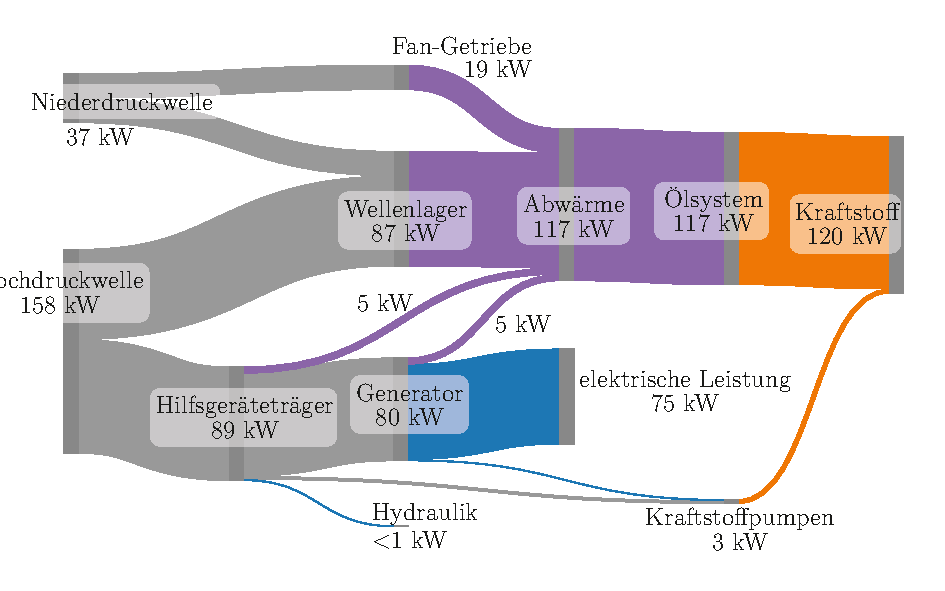
\includegraphics[width=1\linewidth]{4_Abbildungen/2_Hauptteil/sankey.pdf}
	\caption{Abwärmequellen des Kerosin-Kraftstoffsystems}
	\label{fig:sankey}
\end{figure}
\FloatBarrier 


Brewer \cite{Brewer.1991} hat für das Kabinen-Klimasystem (ECS) eines Schmalrumpfflugzeugs eine Abwärme pro Triebwerk von \SI{32}{\kilo\W} berechnet. Dieser Wert wird für die Modellierung übernommen. Durch das Kabinen-Klimasystem steht den Wasserstoff-Kraftstoffsystemen eine höhere Abwärme von insgesamt $\dot{Q}_{\mathrm{FOHE}}=$ \SI{149}{\kilo\W} zur Verfügung.

\section{Pumpen und Verdichter}

\subsection{Kreiselpumpen}

Kreiselpumpen kommen im Kerosin-Kraftstoffsystem als Niederdruckpumpe und im Wasserstoff-Kraftstoffsystem mit Pumpe als Hochdruckpumpe zum Einsatz. Kreiselpumpen erreichen ihren maximalen Wirkungsgrad bei mittleren Volumenströmen und hohen Druckverhältnissen, beziehungsweise Drehzahlen \cite{Gulich.2013}. %Ein typisches Kennfeld einer Kreiselpumpe ist in Abbildung \ref{fig:kreiselpumpe} dargestellt.

%\begin{figure}[ht]
%\centering
%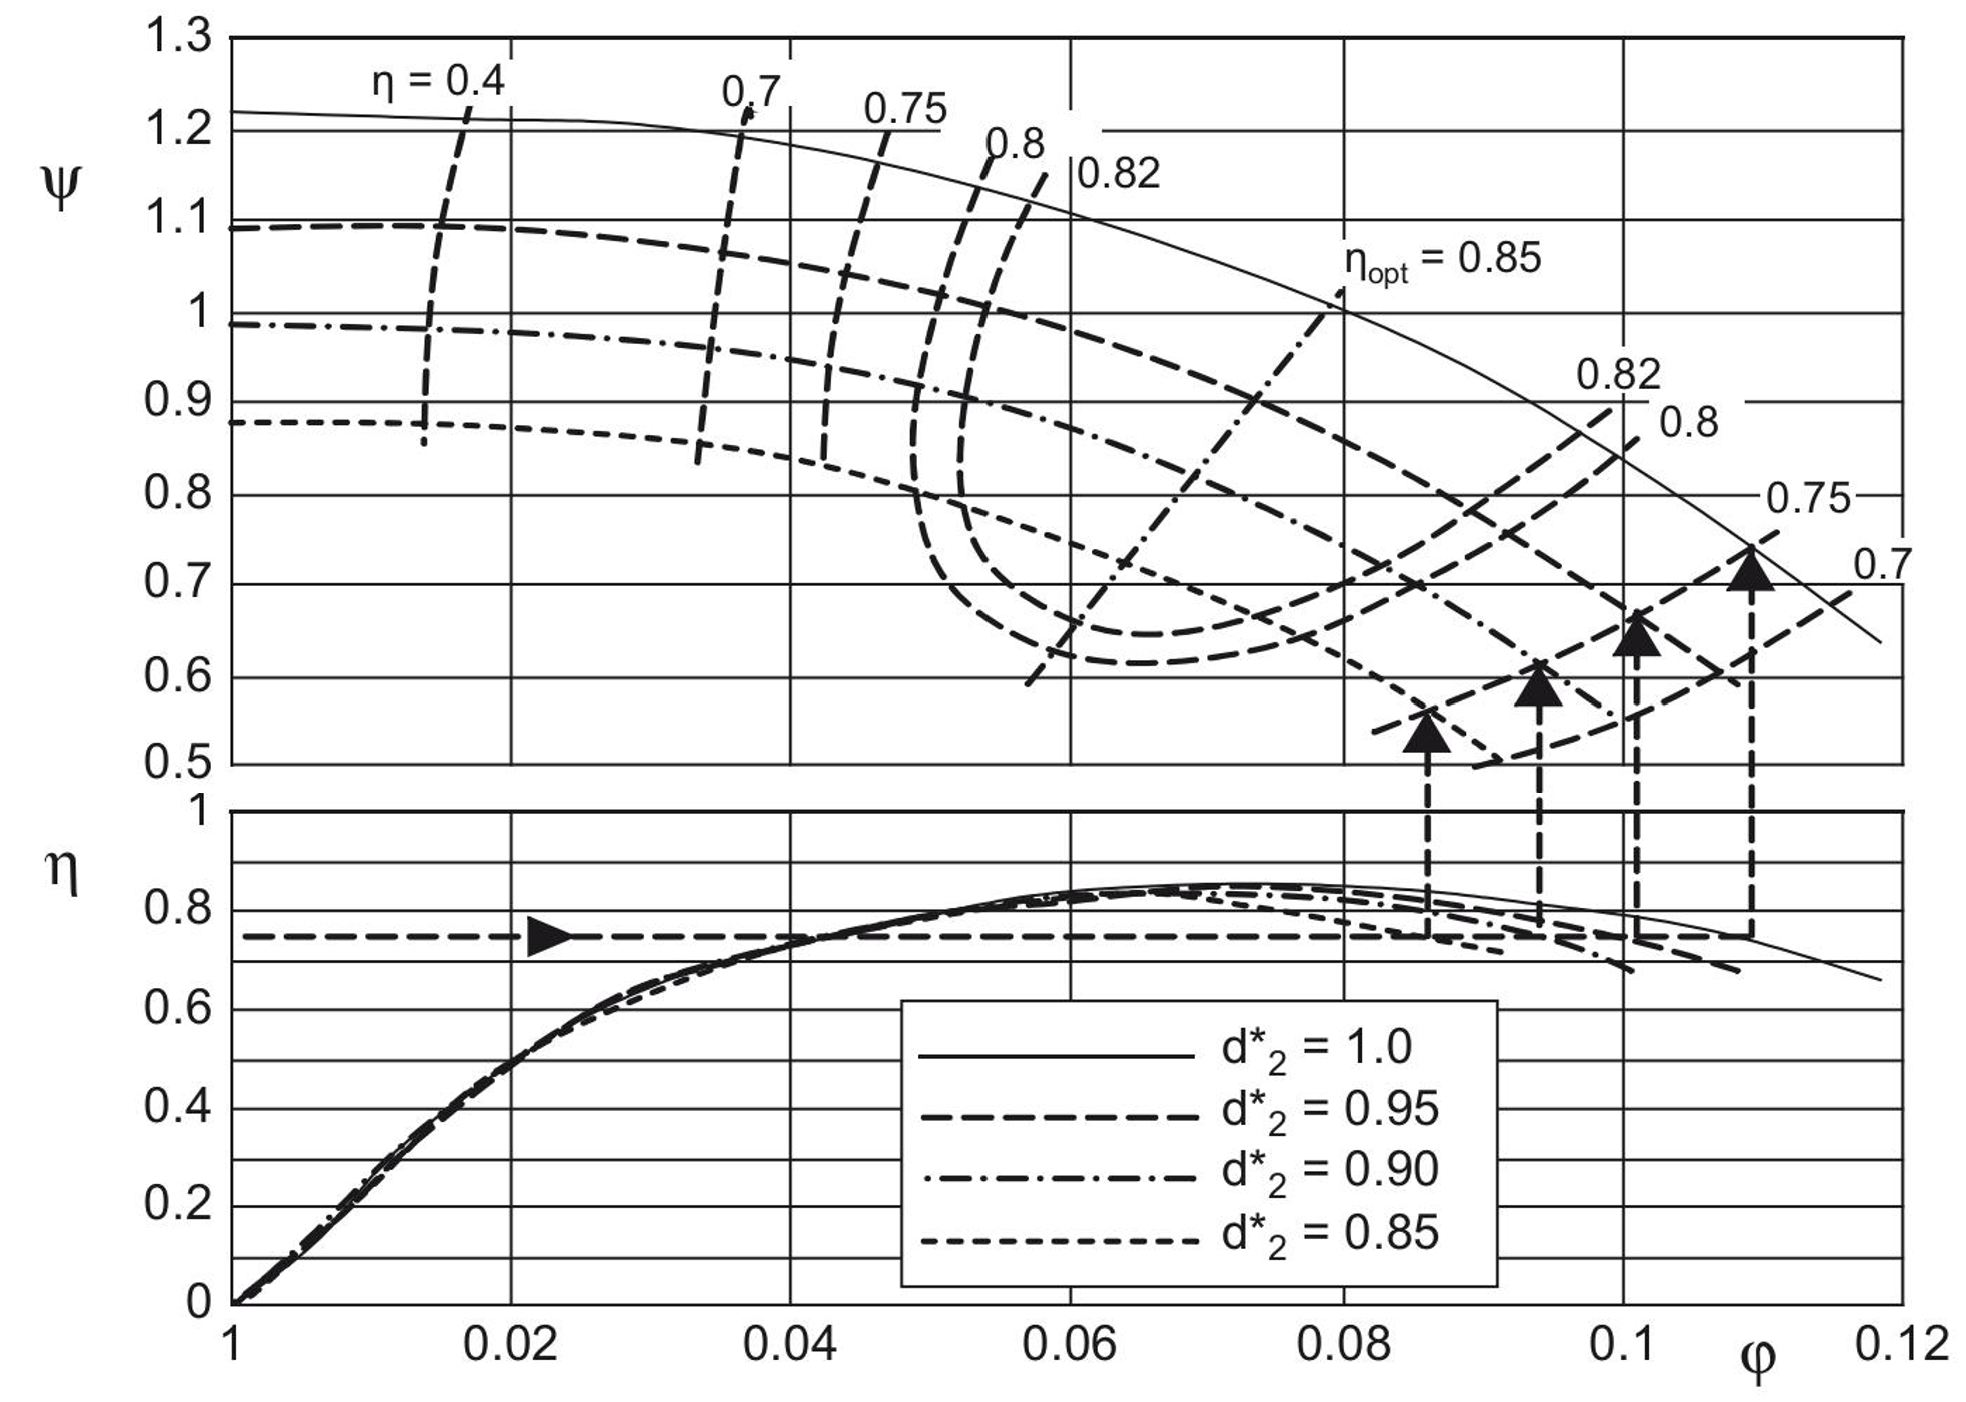
\includegraphics[width=0.8\linewidth]{4_Abbildungen/2_Hauptteil/kreiselpumpe.png}
%  \caption{Kennfeld einer Kreiselpumpe \cite{Gulich.2013}}
%  \label{fig:kreiselpumpe}
%\end{figure}
%\FloatBarrier 

Die Niederdruckpumpen von Kerosin-Kraftstoffsystemen erreichen im Reiseflug aufgrund der niedrigeren Drehzahlen und Volumenströmen im Vergleich zum optimalen Betriebspunkt nur vergleichsweise niedrige Wirkungsgrade zwischen $53$ und $66\,\%$ \cite{Zhou.2023}. Für die Niederdruckpumpe des Kerosin-Kraftstoffsystems wird ein isentroper Wirkungsgrad von $\eta_{\mathrm{LP}}=0,60$ angenommen. Die Niederdruckpumpe des CFM56-5B erzeugt im Auslegungspunkt eine Druckerhöhung von $\Delta p_{\mathrm{MTO}}=$ \SI{965}{\kilo\Pa}. Gemäß den Ähnlichkeitsbeziehungen für Pumpen \cite{Gulich.2013} beträgt der Austrittsdruck $p_{LP}$ 

\begin{equation}\label{Eq:lpfp}
	p_{\mathrm{LP}}=p_e+\Delta p_{\mathrm{MTO}}\left(\frac{N_2}{N_{2,\mathrm{MTO}}}\right)^2
\end{equation}

der Niederdruckpumpe im Reiseflug somit \SI{930}{\kilo\Pa}.

Da Wasserstoff-Kraftstoffsysteme keine nennenswerten Kraftstoffmassenströme in die Kraftstofftanks rückführen können, fallen die Volumenströme im Reiseflug relativ zu MTO-Bedingungen nochmals geringer aus als bei Kerosin-Kraftstoffsystemen. Brewer \cite{Brewer.1991} berechnet für den Wirkungsgrad einer Hochdruckpumpe mit konstanter Übersetzung im Wasserkraftstoffsystem einen Wert von $\eta_{\mathrm{HP}}=0,154$. Mit variabler Übersetzung sind höhere Wirkungsgrade möglich, jedoch verursachte diese Lösung höhere Betriebskosten und wird daher nicht betrachtet \cite{Brewer.1991}. 

\subsection{Zahnradpumpen}

Xu et al. \cite{Xu.2024} haben den Wirkungsgrad einer Zahnrad-Hochdruckpumpe bei unterschiedlichen Drehzahlen untersucht. Hohe Drehzahlen ermöglichen hohe Wirkungsgrade von bis zu $0,78$. Die Hochdruckpumpe des CFM56-5B arbeitet mit einer Nenndrehzahl von $6250$ 1/min \cite{EatonFuelSystemsDivision.2008}. Da die Hochdruckpumpe mit einem konstanten Übersetzungsverhältnis an die Hochdruckwelle angeschlossen ist, beträgt die Drehzahl im Reiseflug (mit $N_2/N_{2,\mathrm{MTO}}=0,88$) $5500$ 1/min. Interpolation der Daten von Xu et al. \cite{Xu.2024} ergibt somit einen Wirkungsgrad der Hochdruckpumpe von $\eta_{\mathrm{HP}}=0,73$.

Für die Hochdruckpumpe wird zudem der geförderte Massenstrom festgelegt. Unter MTO-Bedingungen fördert die Hochdruckpumpe den Kraftstoffverbrauch von \SI{1.05}{\kg\per\s} zuzüglich Kontingenz. Bei einem angenommenen Überschuss von $20\,\%$, beträgt der geförderte Massenstrom bei MTO-Schub \SI{1.27}{\kg\per\s}. Unter Annahme einer identischen volumetrischen Effizienz in beiden Lastpunkten beträgt der geförderte Massenstrom im Reiseflug aufgrund der niedrigeren Drehzahl somit $\dot{m}_\mathrm{HP}=$ \SI{1.11}{\kg\per\s}.

\subsection{Wasserstoff-Verdichter}

Der im Reiseflug gegenüber MTO-Bedingungen stark verringerte Volumenstrom bei nur geringfügig verringerter Drehzahl würde bei konstantem Übersetzungsverhältnis eine erhebliche Pumpgefahr bedeuten. Um einen stabilen Betrieb mit hohem Wirkungsgrad zu gewährleisten ist daher eine variable Übersetzung zwischen Verdichter und der Hochdruckwelle des Verdichters notwendig. 

Bei einem angenommenen Teillast-Wirkungsgrad des Verdichters von $0,75$ und einem mechanischen Wirkungsgrad der variablen Übersetzung von $0,95$ beträgt der Gesamtwirkungsgrad $\eta_{\mathrm{HP}}=\eta_\mathrm{RV}=0,71$.

\section{Wärmeübertrager Druckverluste}

Bei der Auslegung von Wärmeübertragern wird ein Kompromiss zwischen Bauvolumen/Masse und Druckverlust angestrebt. Da Masse und Bauvolumen der Kraftstoffsysteme in dieser Arbeit nicht berücksichtigt werden, erfolgt keine konkrete Auslegung der Wärmeübertrager, etwa mit der NTU-Methode. Stattdessen werden die Druckverluste anhand von Erfahrungswerten abgeschätzt. Für die Wasserstoff-Kraftstoffsysteme werden die Druckverluste in den Wärmeübertragern mit der parallelen Wasserstoffverbrennung, dem Klimasystem und dem Hauptölsystem sowie des Verdampfer bestimmt. Für das Kerosin-Kraftstoffsystem wird ausschließlich der Druckverlust im Wärmeübertrager des Hauptölsystem ermittelt.

\subsection{Kerosin-Kraftstoffsystem}

Zu den kraftstoffseitigen Druckverlusten in Wärmeübertragern von Kerosin-Kraftstoffsystemen liegen in der Literatur keine zuverlässigen Angaben vor, daher wird der Wert geschätzt. Einerseits sind bei Kerosin-Wärmeübertragern aufgrund der höheren Viskosität von Kerosin im Vergleich zu gasförmigem Wasserstoff sowie der geringeren Temperaturdifferenz der Fluidströme höhere Druckverluste zu erwarten. Andererseits überträgt der FOHE-Wärmeübertrager des Kerosin-Kraftstoffsystems aufgrund des höheren Massenstroms eine geringere spezifische Wärme als die der Wasserstoff-Kraftstoffsysteme. Zudem ermöglicht die deutlich höhere Dichte von Kerosin gegenüber gasförmigem Wasserstoff bei konstantem Flächen-zu-Massenstrom-Verhältnis niedrigere Strömungsgeschwindigkeiten, was geringere Druckverluste ermöglichen kann. Unter diesen Abwägungen wird für den FOHE-Wärmeübertrager des Kerosin-Kraftstoffsystems ein Druckverhältnis von $0,95$ angenommen.

\subsection{Wasserstoff-Kraftstoffsysteme}

Sciatti et al. \cite{Sciatti.2025} haben einen Wärmeübertrager zwischen Wasserstoff und Stickstoff untersucht und ausgelegt. Im Vergleich zum PHC-Wärmeübertrager der Wasserstoff-Kraftstoffsysteme dieser Arbeit sind die Temperaturdifferenz der Fluidströme geringer und die übertragene spezifische Wärme höher. Das von Sciatti et al. ermittelte Druckverhältnis über den Wärmeübertrager von $0,988$ stellt daher eine konservative Abschätzung der Druckverluste des PHC-Wärmeübertragers dar. Jedoch hat der ausgelegte Wärmeübertrager eine für den Wasserstoff-Massenstrom korrigierte Masse von \SI{111}{\kg} und ist damit inakzeptabel schwer. Für den PHC-Wärmeübertrager der Wasserstoff-Kraftstoffsysteme wird ein Druckverhältnis von $0,98$ angenommen.

Brewer \cite{Brewer.1991} hat für einen Wasserstoff Wärmeübertrager mit dem Kabinen-Klimasystem Druckverluste von \SI{2.14}{\kilo\Pa} berechnet. Die vernachlässigbar geringen Druckerverluste resultieren aus der geringen übertragenen Wärme bei moderater Temperaturdifferenz.

Für einen Wasserstoff-Wärmeübertrager mit dem Hauptölsystem hat Brewer ein Druckverhältnis von $0,984$ von berechnet \cite{Brewer.1991}. Die Wärmeübertrager mit den Hauptölsystemen der Wasserstoff-Kraftstoffsysteme dieser Arbeit übertragen das Vierfache der spezifischen Wärme. Die Übertragung der höheren spezifischen Wärme erfordert zusätzliche Rohrreihen im Wärmeübertrager. Da der Druckverlust unterproportional mit der Anzahl an Reihen skaliert \cite{.2013b}, erscheint ein Druckverhältnis über den Wärmeübertrager von $0,95$ realisierbar. Da die Druckverluste des Wärmeübertragers mit dem Klimasystem vernachlässigbar sind, ergibt sich für beide Wärmeübertrager in Summe ein Druckverhältnis von $\pi_{\mathrm{FOHE}}=0,95$.

Sciatti et al. \cite{Sciatti.2025} haben einen Wärmeübertrager für die Verdampfung von Flüssigwasserstoff mit erwärmtem Wasserstoff ausgelegt. Sie haben Druckverluste von \SI{5.74}{\Pa} für die heiße Seite und \SI{10.2}{\Pa} für die kalte Seite berechnet. Die vernachlässigbar geringen Druckverluste resultieren aus der hohen Temperaturdifferenz der Wasserstoff-Massenströme und der vergleichsweise geringen übertragenen Wärme. Für das Wasserstoff-Kraftstoffsystem mit Verdampfer werden daher die Druckverhältnisse $\pi_{\mathrm{V,LP}}=\pi_{\mathrm{V,HP}}=1$ angenommen.

\section{Leitungs- und Injektor-Druckverluste}

Die Leitungen der Kraftstoffsysteme verursachen Druckverluste infolge von Rohrreibung. Zudem erfordern die Injektoren eine minimale Druckdifferenz zwischen Kraftstoffzufuhr und Brennkammer, um eine adäquate Zerstäubung des Kraftstoffs zu gewährleisten.

\subsection{Kerosin-Kraftstoffsystem}

Die Rohrreibungsverluste im Kerosin-Kraftstoffsystem $\Delta p_\mathrm{L}$ 

\begin{equation}\label{Eq:dp}
	\Delta p_\mathrm{L}=\lambda\frac{L}{D}\frac{\rho}{2}v^2
\end{equation}

werden mit der Darcy-Weisbach-Gleichung bestimmt. Hierbei werden der Rohrreibungswert $\lambda=0,025$, die Leitungslänge $L=$ \SI{0.5}{\m}, der Leitungsdurchmesser $D=$ \SI{14}{\milli\m}, die Kraftstoffdichte $\rho=$ \SI{760}{\kg\per\m\cubed} und die Strömungsgeschwindigkeit $v=$ \SI{10}{\m\per\s} angenommen. Daraus resultiert der Druckverlust $\Delta p_\mathrm{L}=$ \SI{68}{\kilo\Pa}. 

Mazaheri et al. \cite{Mazaheri.2012} haben Drallinjektoren für Luftfahrtanwendungen mit einer Druckdifferenz von $\Delta p_{\mathrm{inj}}=$ \SI{300}{\kilo\Pa} ausgelegt.

\subsection{Wasserstoff-Kraftstoffsysteme}

Die Rohrreibungsverluste der Wasserstoff-Kraftstoffsysteme werden mit der Darcy-Weisbach-Gleichung (Gleichung \ref{Eq:dp}) bestimmt. Hierbei werden der Rohrreibungswert $\lambda=0,02$, die Leitungslänge $L=$ \SI{0.5}{\m}, der Leitungsdurchmesser $D=$ \SI{92}{\milli\m}, die Kraftstoffdichte $\rho=$ \SI{1.33}{\kg\per\m\cubed} und die Strömungsgeschwindigkeit $v=$ \SI{60}{\m\per\s} angenommen. Daraus resultiert der Druckverlust $\Delta p_\mathrm{L}=$ \SI{260}{\kilo\Pa}. 


Brewer \cite{Brewer.1991} hat für ein Wasserstoff-Kraftstoffsystem Injektor-Druckverluste von $p_{\mathrm{inj}}=$ \SI{169}{\kilo\Pa} berechnet. Dieser Wert wird für die Modellierung übernommen.

\section{Parallele Wasserstoffverbrennung}

Die parallele Wasserstoffverbrennung wird als magere Verbrennung mit einem Brennstoff-Luft-Verhältnis von 0,01 modelliert. Für die Verbrennung wird ein unterer Heizwert von Wasserstoff von $H_{u, \mathrm{H}_2}= $ \SI{120}{\mega\J\per\kg} angenommen. Die spezifischen isobaren Wärmekapazitäten von Luft und dem Abgas werden mit dem CEARUN Web-Tool \cite{Leader.} bestimmt. Für die Fan-Zapflufttemperatur wurde ein Wert von \SI{273}{\K} berechnet (Siehe Tabelle \ref{Tab:cruise}). Für die Annäherungstemperatur des PHC-Wärmeübertragers wird ein Wert von $\Delta T= $ \SI{30}{\K} angenommen. %Dieser Wert stellt einen Kompromiss zwischen der Masse des PHC-Wärmeübertragers und dem Gesamtwirkungsgrad dar.

\section{Zusammenfassung}

Die Parameter des Kerosin-Kraftstoffsystems sind in Tabelle \ref{Tab:referenz_parametrisiert} gesammelt.

\begin{table}[ht]
    \centering
	\caption{Randbedingungen des Kerosin-Kraftstoffsystems}
	\begin{tabular} {|l|c|c|c|c|} \hline%
		\multicolumn{2}{|c|}{Parameter} & Einheit & Wert & Quelle\\ \hline\hline%
        LPFP-Eintrittstemperatur & $T_e$ & K & 270 & - \\ \hline
        LPFP-Eintrittsdruck & $p_e$ & kPa & 180 & \cite{EatonFuelSystemsDivision.2013} \\ \hline
        FOHE-Wärme & $\dot{Q}_{\mathrm{FOHE}}$ & kW & 112 & - \\ \hline
        FOHE-Druckverhältnis & $\pi_{\mathrm{FOHE}}$ & - & 0,95 & - \\ \hline
        IDG-FOHE Wärme  & $\dot{Q}_\mathrm{IDG}$ & kW & 5 & \cite{Sciatti.2024} \\ \hline
        LPFP-Austrittsdruck & $p_\mathrm{LP}$ & kPa & 930 & - \\ \hline
        isentroper Wirkungsgrad LPFP & $\eta_\mathrm{LP}$ & - & 0,60 & \cite{Zhou.2023} \\ \hline
        isentroper Wirkungsgrad HPFP & $\eta_\mathrm{HP}$ & - & 0,73 & \cite{Xu.2024} \\ \hline
        HPFP-Massenstrom & $\dot{m}_\mathrm{HP}$ & kg/s & 1,11 & - \\ \hline
        Brennkammer-Massenstrom & $\dot{m}_\mathrm{BK}$ & kg/s & 0,313 & - \\ \hline
        Leitungs-Druckverluste & $\Delta p_\mathrm{L}$ & kPa & 68 & - \\ \hline
        Injektor-Druckverluste & $\Delta p_\mathrm{inj}$ & kPa & 300 & \cite{Mazaheri.2012} \\ \hline
	\end{tabular}	
    \label{Tab:referenz_parametrisiert}%
\end{table}
\FloatBarrier 

Die Parameter der Wasserstoff-Kraftstoffsysteme sind in Tabellen \ref{Tab:h2_parametrisiert} und \ref{Tab:h2_param2} dokumentiert.

\begin{table}[ht]
    \centering
	\caption{Parameter der Modellierungen aller Wasserstoff-Kraftstoffsysteme}
	\begin{tabular} {|l|c|c|c|c|} \hline%
    \multicolumn{5}{|c}{Alle Wasserstoff-Kraftstoffsysteme}\\ \hline
    \multicolumn{2}{|c|}{Parameter} & Einheit & Wert & Quelle\\ \hline\hline%
    isentroper Wirkungsgrad RV & $\eta_\mathrm{RV}$ & - & 0,71 & - \\ \hline
    Kraftstoff-Eintrittsdruck & $p_e$ & kPa & 345 & \cite{Brewer.1991, Scholz.2003} \\ \hline
    Kraftstoff-Eintrittstemperatur & $T_e$ & K & 25,2 & \cite{Brewer.1991, Scholz.2003} \\ \hline
    PHCHE-Druckverhältnis  & $\pi_\mathrm{PHC}$ & - & 0,98 & \cite{Sciatti.2025} \\ \hline
    FOHE-Wärme & $\dot{Q}_\mathrm{FOHE}$ & kW & 149 & - \\ \hline
    FOHE-Druckverhältnis & $\pi_\mathrm{FOHE}$ & - & 0,95 & \cite{Brewer.1991} \\ \hline
    Brennkammer-Massenstrom & $\dot{m}_{\mathrm{BK}}$ & kg/s & 0,110 & - \\ \hline
    Leitungs-Druckverluste & $\Delta p_\mathrm{L}$ & kPa & 260 & \cite{Brewer.1991} \\ \hline
    Injektor-Druckverluste & $\Delta p_\mathrm{inj}$ & kPa & 169 & \cite{Brewer.1991} \\ \hline
    PHC-Brennstoff-Luft-Verhältnis & $\beta_\mathrm{PHC}$ & - & 0,01 & - \\ \hline
    isobare Wärmekapazität Luft & $c_{p, \mathrm{L}}$ & \si{\kilo\J\per\kg\per\K} & 1,0 & \cite{Leader.} \\ \hline
    isobare Wärmekapazität Abgas & $c_{p, \mathrm{B}}$ & \si{\kilo\J\per\kg\per\K} & 1,1 & \cite{Leader.} \\ \hline
    unterer Heizwert Wasserstoff & $H_{u, \mathrm{H}_2}$ & MJ/kg & 120 & - \\ \hline
    PHCHE-Annäherungstemperatur & $\Delta T$ & K & 30 & - \\ \hline
    Fan-Zapflufttemperatur & $T_{13}$ & K & 273 & - \\ \hline
   
    \end{tabular}	
    \label{Tab:h2_parametrisiert}%
\end{table}
\FloatBarrier 

\begin{table}[ht]
	\centering
	\caption{Parameter der Modellierungen der einzelnen Wasserstoff-Kraftstoffsysteme}
	\begin{tabular} {|l|c|c|c|c|} \hline%	
		\multicolumn{5}{|c|}{Architektur mit Hochdruckpumpe}\\ \hline
		\multicolumn{2}{|c|}{Parameter} & Einheit & Wert & Quelle\\ \hline\hline%
		isentroper Wirkungsgrad HPFP & $\eta_\mathrm{HP}$ & - & 0,154 & \cite{Brewer.1991} \\ \hline
		\multicolumn{5}{|c|}{Architektur mit Verdampfer}\\ \hline
		\multicolumn{2}{|c|}{Parameter} & Einheit & Wert & Quelle\\ \hline\hline%
		isentroper Wirkungsgrad HPFC & $\eta_\mathrm{HP}$ & - & 0,71 & - \\ \hline
		Druckverhältnis LP-Verdampfer & $\pi_\mathrm{V,LP}$ & - & 1 & \cite{Sciatti.2025} \\ \hline
		Druckverhältnis HP-Verdampfer & $\pi_\mathrm{V,HP}$ & - & 1 & \cite{Sciatti.2025} \\ \hline\hline
		\multicolumn{5}{|c|}{Architektur mit Vormischung}\\ \hline
		\multicolumn{2}{|c|}{Parameter} & Einheit & Wert & Quelle\\ \hline\hline%
		isentroper Wirkungsgrad HPFC & $\eta_\mathrm{HP}$ & - & 0,71 & - \\ \hline
	\end{tabular}	
	\label{Tab:h2_param2}%
\end{table}
\FloatBarrier 

\section{Brennkammereintritts-Bedingungen}

Im Folgenden werden die unabhängigen Variablen, also die Brennkammer-Eintrittsbedingungen der Kraftstoffsysteme, erläutert. Zunächst wird der Brennkammerdruck der Kraftstoffsysteme festgelegt. Anschließend wird die zulässige Brennkammer-Eintrittstemperatur für das Kerosin-Kraftstoffsystem bestimmt. Zuletzt werden denkbare Wertebereiche für die Betrachtung der Brennkammer- und Wärmeübertrager-Eintrittstemperaturen der Wasserstoff-Kraftstoffsysteme in einer Parameterstudie bestimmt.

\subsection{Brennkammerdruck}

Der Brennkammerdruck beträgt sowohl für das Kerosin- als auch die Wasserstoff-Kraftstoffsysteme $p_\mathrm{BK}=p_3=$ \SI{1330}{\kilo\Pa} (siehe Tabelle \ref{Tab:cruise}).

\subsection{Brennkammer-Eintrittstemperatur Kerosin-Kraftstoffsystem}

Um im Kerosin-Kraftstoffsystem geringere Brennkammer-Eintrittstemperatur zu erreichen, muss eine größere Menge an Kraftstoff in die Kraftstofftanks rückgeführt werden. Um den rückgeführten Kraftstoff zu ersetzen fördert die Niederdruckpumpe einen höheren Kraftstoffmassenstrom, was ihren Leistungsbedarf steigert. Aus diesem Grund wird eine möglichst hohe Brennkammer-Eintrittstemperatur angestrebt. 

Der Brennkammer-Eintrittstemperatur ist jedoch durch die maximal zulässige Öltemperatur eine technische Obergrenze gesetzt. Der Kraftstoff kann nur bis zu der maximalen Öltemperatur abzüglich der Annäherungstemperatur des Wärmeübertragers erhitzt werden. Bei dem PW1133G Triebwerk beträgt die maximale Öltemperatur im Reiseflug \SI{419}{\K} \cite{EASA.2018}. Bei einer angenommenen Annäherungstemperatur zuzüglich Kontingenz von \SI{20}{\K} beträgt die maximal zulässige Brennkammer-Eintrittstemperatur somit $T_\mathrm{BK}=$ \SI{399}{\K}.

\subsection{Eintrittstemperaturen Wasserstoff-Kraftstoffsysteme}

Das EnableH2 Projekt \cite{Patrao.2023} sowie Brewer \cite{Brewer.1991} gehen von Brennkammer-Eintrittstemperaturen von über \SI{650}{\K} aus. Diese hohen Temperaturen erreichen die Autoren insbesondere durch den Einsatz von Wärmerückgewinnung aus dem Abgas des Kerntriebwerks. Die Autoren des CRYOPLANE Berichts \cite{Scholz.2003} und der Joint Cryogenic Engine Study \cite{SIMON.1994} halten Wasserstofftemperaturen von \SI{150}{\K} für ausreichend. Tacconi et al. \cite{Tacconi.2023} haben für ihre Betrachtung eines Wasserstoff-Kraftstoffsystems eine minimale akzeptable Temperatur von \SI{273}{\K} angenommen, um Probleme infolge von Vereisung in der Brennkammer zu vermeiden. Aufgrund der breiten Palette an Vorschlägen für Brennkammer-Eintrittstemperaturen für Wasserstoff-Kraftstoffsysteme wird diese Variable in der Parameterstudie in einem Wertebereich zwischen $150$ und \SI{500}{\K} untersucht. Für den Vergleich mit dem Kerosin-Kraftstoffsystem wird ein Wert von \SI{300}{\K} verwendet.

Ähnliches gilt für die Wärmeübertrager-Eintrittstemperatur. Um Vereisungen in den Öl- und Luftwärmeübertragern zu vermeiden, wird eine minimale Eintrittstemperatur gewahrt. Wärmeübertrager-Eintrittstemperaturen oberhalb des Gefrierpunkts von Wasser sind jedoch nicht sinnvoll, da dort keine Vereisungsgefahr mehr besteht und eine weitere Erhöhung der Temperatur lediglich den rezirkulierten Massenstrom erhöhen würde. Der Wärmeübertrager-Eintrittstemperatur ist jedoch durch die Brennkammer-Eintrittstemperatur eine weitere Obergrenze gesetzt. Damit exzessive rezirkulierte Massenströme vermieden werden, wird stets eine Wärmeübertrager-Eintrittstemperatur gewählt, die mindestens \SI{20}{\K} unter der Brennkammer-Eintrittstemperatur liegt. Die Wärmeübertrager-Eintrittstemperatur wird im Rahmen der Parameterstudie in einem Wertebereich zwischen $100$ und \SI{280}{\K} untersucht. Für den Vergleich mit dem Kerosin-Kraftstoffsystem wird ein Wert von \SI{160}{\K} verwendet.

